\chapter{Resultados}
\label{cap:resultados}
%\todo[inline]{Em todas as figuras em que aparecem os gráficos das 5 execuções, eu troquei o width=0.8\textwidth por width=\textwidth, porque os textos nelas estavam muito pequenos, impossíveis de ler sem zoom.}

Neste capítulo, são apresentados os resultados dos experimentos de avaliação do \texttt{CEP Handler} descritos no Capítulo~\ref{cap:experimento}. Foram executados dez experimentos no total, cinco repetições para cada um dos dois algoritmos de balanceamento de carga apresentados na Seção~\ref{sec:loadDistribution}. 

As seções a seguir discutem os dados detectados relevantes no contexto de monitoramento de tráfego de ônibus na cidade de São Paulo, bem como o custo computacional e as medidas de desempenho (tais como número total, vazão e latência de eventos detectados) por execução do experimento. 
Ao final do capítulo, são apresentadas as conclusões dos resultados e uma discussão sobre os efeitos do uso de cada um dos algoritmos de balanceamento de carga. 

\section{Dados Detectados}

Como discutido no Capítulo \ref{cap:experimento}, os tipos de eventos do cenário do experimento foram escolhidos com o propósito de criar uma rede de processamento de eventos grande o suficiente para avaliar o funcionamento da auto-escalabilidade do \texttt{CEP Handler}, como é o caso da rede de detecção de problemas de tráfego de ônibus de São Paulo.
Os tipos de eventos nas pontas da rede da Figura~\ref{fig:experiment_diagram}, especificamente a detecção de agrupamento de ônibus e a detecção de velocidade média em corredor de ônibus principal, servem o propósito de verificar se a frota de ônibus está circulando como o determinado pelo planejamento da SPTrans. 

%As principais informações que foram retiradas a partir dos dados da SPTrans, se referiam a detecção de agrupamento de ônibus em tempo real e a detecção da velocidade média em cada corredor de ônibus na cidade. 
Os gráficos das figuras \ref{fig:avg_speed_guara_1} e \ref{fig:histogram_Bus_Bunching} foram criados a partir dos dados das detecções desses tipos de eventos em uma das execuções do experimento. A Figura  \ref{fig:avg_speed_guara_1} mostra as velocidades médias detectadas no corredor de ônibus Guarapiranga. Os gráficos das velocidades médias dos outros 11 corredores de ônibus principais da cidade podem ser encontrados no Apêndice \ref{ape:graphics}. A Figura \ref{fig:histogram_Bus_Bunching} mostra o número de ocorrências de agrupamentos de ônibus dentro de intervalos de 15 minutos, ao longo de todo o período de circulação de ônibus coberto pelo experimento. De uma execução para outra do experimento, não houve variação significativa nos eventos detectados pelo sistema \texttt{CEP Handler}, como era esperado. 
% Kelly: reescrito acima
%A partir das detecções desses tipos de eventos, foi possível criar um histograma com o número de ocorrências de agrupamentos de ônibus dentro de intervalos de quinze minutos, mostrado Figura \ref{fig:histogram_Bus_Bunching} e das velocidades médias de cada um dos doze corredores de ônibus, um dos quais está representado na figura  \ref{fig:avg_speed_guara_1}. Estes e os gráficos da velocidade média dos outros corredores de ônibus podem ser encontradas no Apêndice \ref{ape:graphics}. 

% Kelly: reescrito acima
%Apesar de apresentarem os resultados práticos da detecção de eventos, as informações representadas nestas figuras não é diretamente relevante para a análise do funcionamento do sistema cep handler, especialmente pois os dados utilizados para a geração dos gráficos não foram significativamente diferentes entre uma execução e outra do experimento. 

O gráfico da Figura \ref{fig:avg_speed_guara_1} mostra a velocidade pelo horário de coleta do dado. 
Como explicado na Seção~\ref{sec:exp_event_types}, a velocidade média de um corredor é calculada pelos tipos de evento da categoria \textbf{vi}, a partir das velocidades médias dos ônibus que passam no corredor nos últimos cinco minutos.
O gráfico mostra uma discrepância entre as velocidades detectadas nos minutos iniciais e as velocidades detectadas posteriormente. Isso se deve ao fato de que, nos primeiros minutos, as janelas de agregação para o cálculo das velocidades médias não agregam dados suficientes,  pois ainda não se passaram os cinco minutos necessários para o cálculo. Ao longo de todo o período do experimento, a velocidade média móvel do corredor Guarapiranga se manteve majoritariamente entre os 30 km/h e 50 km/h, um intervalo que deve representar o tráfego comum do corredor. Com esse tipo de evento em atuação, poderia-se detectar em tempo real acidentes nos quais os veículos envolvidos bloqueassem a circulação no corredor.

%Kelly: reescrevi acima
%No gráfico da Figura \ref{fig:avg_speed_guara_1}, que apresenta a velocidade média dos últimos cinco minutos pelo o horário de coleta do dado, é possível observar que o início do gráfico apresenta uma discrepância em relação a velocidade detectada posteriormente. Ao longo de todo o gráfico a velocidade média do corredor se mantêm entre os 35 km/h e 45 km/h, um intervalo que deve representar o funcionamento comum deste corredor. Com este tipo de evento em atuação, poderia-se detectar em tempo real acidentes nos quais os veículos envolvidos bloqueassem a circulação no corredor.


\begin{figure}[h!]
 \centering
 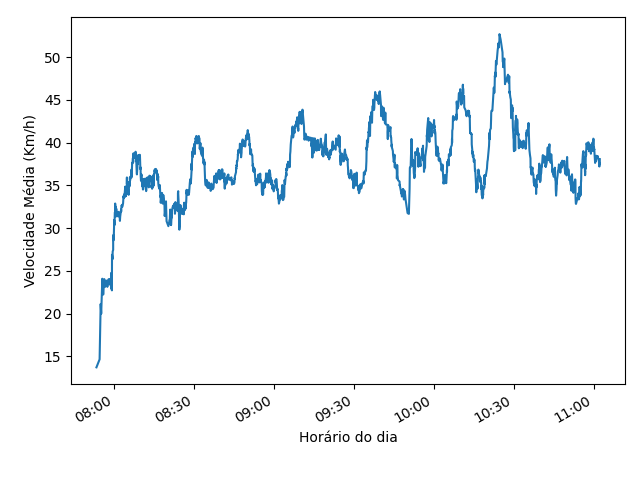
\includegraphics[width=0.6\textwidth]{figuras/detect_graphics/avg_speed_7-dez-su-corr_Guarapiranga.png}
 \caption{Velocidades médias no corredor de ônibus Guarapiranga para uma execução do experimento.}
 \label{fig:avg_speed_guara_1}
\end{figure}

\begin{figure}[h!]
\centering
  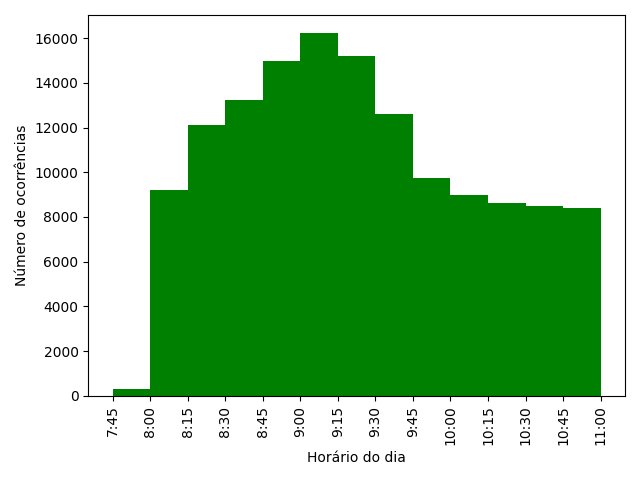
\includegraphics[width=0.6\textwidth]{figuras/detect_graphics/histogram_7-dez-su_BB.png}
  \caption{Histograma do número de ocorrências de agrupamento de ônibus para uma execução do experimento.}
  \label{fig:histogram_Bus_Bunching}
\end{figure}


%\todo[inline]{Fernando, gráficos que não são comparáveis entre si, ou que não são analisados juntos no texto, como é caso das Figuras 7.1 e 7.2, não devem ficar lado a lado. Na dissertação, você não precisa economizar espaço, deve prezar a legibilidade. :)}

%\todo[inline]{No gráfico da Figura 7.2 remover a legenda da linha que aparece no canto superior esquerdo, ela não é necessária.}


O histograma dos eventos de agrupamento de ônibus (Figura~\ref{fig:histogram_Bus_Bunching}) apresenta o número de ocorrências desse tipo a cada intervalo de quinze minutos, utilizando o horário de coleta do dado. Os primeiros dados foram enviados ao sistema às 07h58. Por isso, o  intervalo inicial do histograma, que vai das 7h45 às 8h00, contém um número de ocorrências bem menor do que o dos intervalos seguintes.
É possível observar um crescimento do número de ocorrências até atingir um pico entre às 9h00 e 9h15, sendo que essa faixa de tempo coincide com o maior crescimento do número de dados entrando no sistema (mostrado na Figura~\ref{fig:load_and_instances-time-SU}). Uma possível explicação é que, ao longo da manhã, o número de ônibus ativos em cada linha aumenta. Quando esses ônibus iniciam sua circulação e começam a enviar suas posições para a SPTrans, eles estão localizados em terminais ou garagens, junto com outros ônibus da mesma linha. Depois das 9h15, há uma diminuição do número de ocorrências de aglomeração, pois a maioria dos ônibus está em circulação nas vias, longe de outros ônibus da sua própria linha. A partir das 10h00, a maioria das ocorrências de agrupamento de ônibus detectadas podem ser em terminais de ônibus, onde os veículos ficam estacionados entre uma viagem e outra. 

\section{Auto-Escalabilidade do Sistema}
\label{sec:auto_scalability}
%\todo[inline]{As figuras desta seção estão erradas. As figura 7.3 e 7.4 são iguais. E as figuras 7.5 e 7.6 também são iguais. Além disso, as 2 últimas não são do mesmo experimento das 2 anteriores.}


%\todo[inline]{Não faz sentido comparar lado a lado uma execução do alg 1 com uma execução do alg 2, como você está fazendo nas figuras desta seção. Há 5 x 5 pares desses possíveis. Por que esse par de execuções que você mostrou aqui é o que melhor representa o comportamento dos dois algoritmos? É melhor você mostrar os gráficos das 10 execuções, dividindo eles em duas grandes figuras: uma só com as execuções do alg 1 e outra com as execuções do alg 2. Depois que você incluir essas figuras, é preciso ajustar as discussões do texto para fazer referência a elas.}

%\todo[inline]{Os gráficos que precisam ser analisados juntos devem ficar dentro de um só Figure, mas em Subfigures diferentes. Dessa forma, a apresentação fica melhor e dá para colocar um caption pra figura todo e captions separados para cada subfigura. Veja como usar os subfigures em \url{https://shantoroy.com/latex/add-subfig-in-latex/.}. Por exemplo, as figuras 7.3 e 7.4 deveriam ser uma só figure, com dois subfigures (com os captions atuais). Então, o caption do figure poderia ser algo como ``Número de eventos entrando no sistema no sistema e número de instâncias de \texttt{CEP Worker} em função do tempo em duas execuções do experimento''. }



%\todo[inline]{Nas figuras 7.3 e 7.4, o rótulo do eixo está em inglês (time), precisa ser traduzido. No rótulo do eixo y da direita, está escrito ``número de workers''. Nas figuras 7.5 e 7.6, você chamou de ``número de instâncias''. Nas 4 figuras, seria melhor chamar de ``número de instâncias de cep-worker''.}

%\todo[inline]{Em todos os gráficos, remover a legenda da linha azul, ela não é necessária.}

A partir dos dados coletados de cada repetição do experimento, para os dois algoritmos de balanceamento de carga, foi possível observar que o sistema se auto-escala conforme o número de eventos de entrada aumenta. As figuras \ref{fig:workers_and_events_SU}  e \ref{fig:workers_and_events_IS} mostram o número de instâncias de \texttt{CEP Workers} no sistema ao longo do tempo para todas as execuções do experimento com o algoritmo de balanceamento por Uso de Estado e com o algoritmo de balanceamento por Similaridade de Entrada, respectivamente. 
Em todas, observa-se que o número de instâncias aumenta mesmo antes do início do envio de eventos, enquanto o sistema ainda está cadastrando os tipos de eventos. Cada cadastro já ocupa um espaço na memória RAM, que cumulativamente gera o disparo da instanciação de novos \texttt{CEP Workers}.

 \afterpage{\clearpage}
\begin{figure}[h!]
\begin{subfigure}{.5\textwidth}
  \centering
  % include second image
  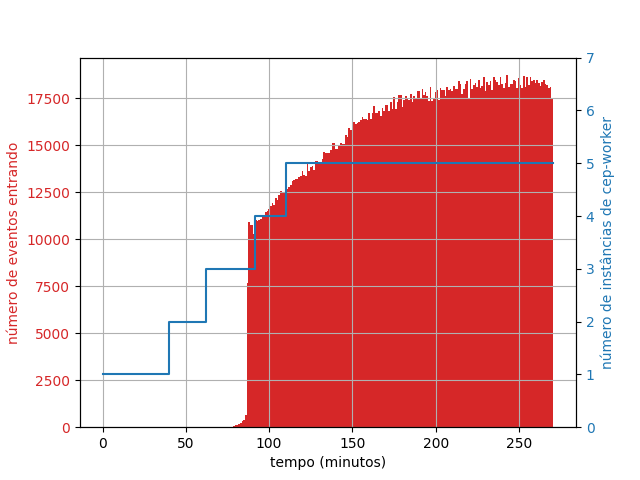
\includegraphics[width=\linewidth]{figuras/graphics/carga_e_workers_total5-dez-su.png}  
  \caption{Execução 1}
  \label{fig:cewt-5-dez-su}
\end{subfigure}
\begin{subfigure}{.5\textwidth}
  \centering
  % include second image
  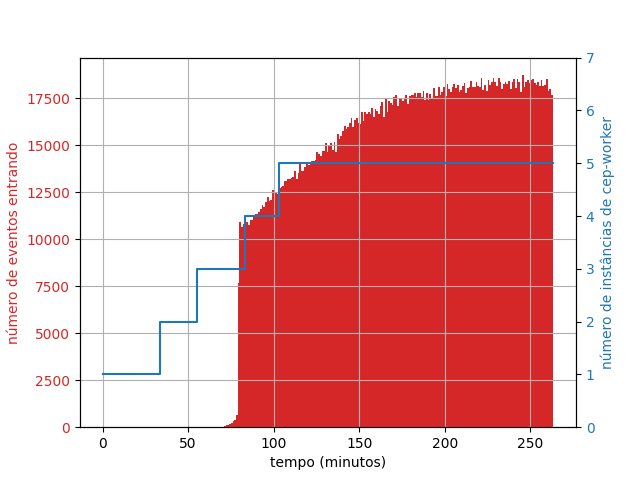
\includegraphics[width=\linewidth]{figuras/graphics/carga_e_workers_total7-dez-su.png}  
  \caption{Execução 2}
  \label{fig:cewt-7-dez-su}
\end{subfigure}
\begin{subfigure}{.5\textwidth}
  \centering
  % include second image
  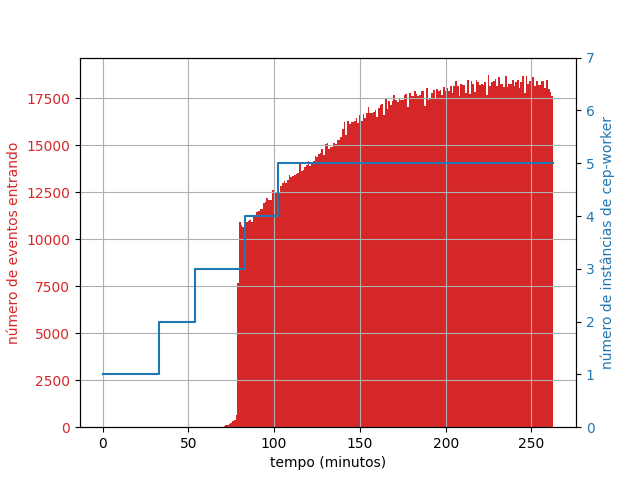
\includegraphics[width=\linewidth]{figuras/graphics/carga_e_workers_total8-dez-su.png}  
  \caption{Execução 3}
  \label{fig:cewt-8-dez-su}
\end{subfigure}
\begin{subfigure}{.5\textwidth}
  \centering
  % include first image
  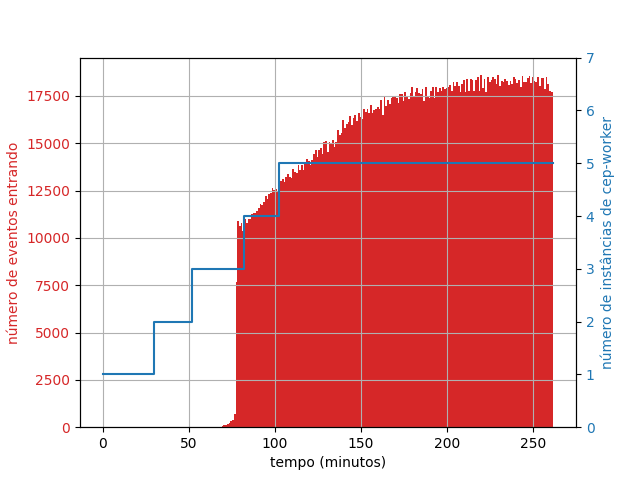
\includegraphics[width=\linewidth]{figuras/graphics/carga_e_workers_total9-dez-su.png}  
  \caption{Execução 4}
  \label{fig:cewt-9-dez-su}
\end{subfigure}
\begin{subfigure}{.5\textwidth}
  \centering
  % include second image
  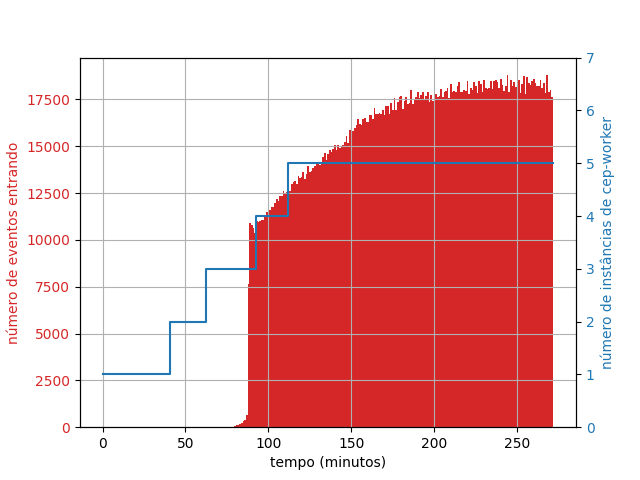
\includegraphics[width=\linewidth]{figuras/graphics/carga_e_workers_total10-dez-su.png}  
  \caption{Execução 5}
  \label{fig:cewt-10-dez-su}
\end{subfigure}
\caption{Número de eventos entrando no sistema (em vermelho) e número de instâncias de \texttt{CEP Worker} (em azul) em função do tempo nas execuções do experimento utilizando o algoritmo de balanceamento de carga por Uso de Estado.}
%\todo[inline]{Fernando, esses gráficos da figura 7.3 estão mesmo certos? Os gráficos das execuções 1 e  5 estão exatamente iguais. O mesmo ocorre com os gráficos das execuções 2 e 3. Isso é estranho. - Sim estão.}
\label{fig:workers_and_events_SU}
\end{figure}

 \afterpage{\clearpage}
\begin{figure}[h!]
\begin{subfigure}{.5\textwidth}
  \centering
  % include second image
  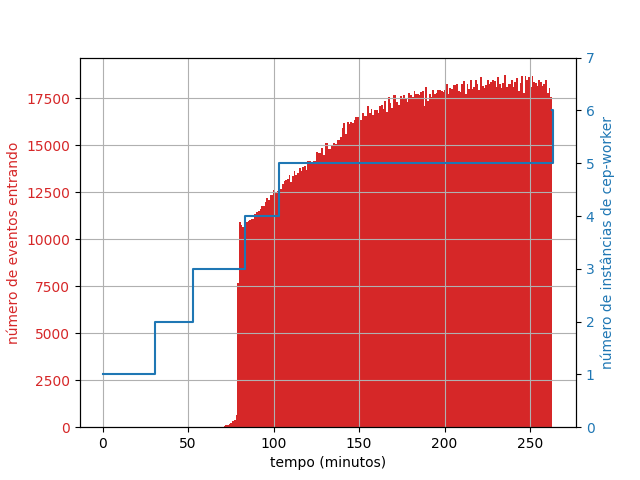
\includegraphics[width=\linewidth]{figuras/graphics/carga_e_workers_total6-dez-is.png}  
  \caption{Execução 1}
  \label{fig:cewt-6-dez-is}
\end{subfigure}
\begin{subfigure}{.5\textwidth}
  \centering
  % include second image
  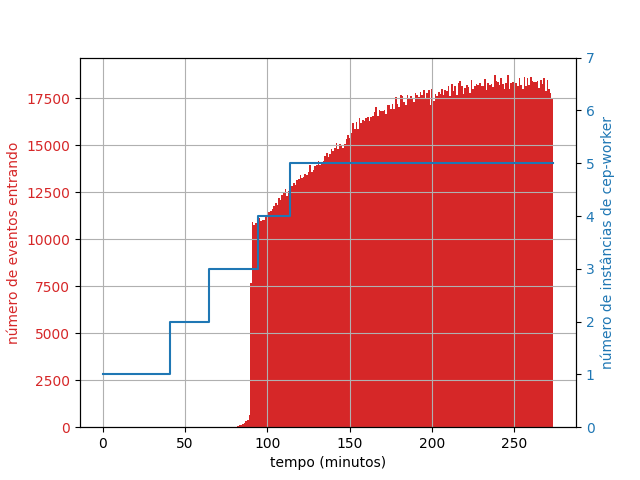
\includegraphics[width=\linewidth]{figuras/graphics/carga_e_workers_total7-dez-is.png}  
  \caption{Execução 2}
  \label{fig:cewt-7-dez-is}
\end{subfigure}
\begin{subfigure}{.5\textwidth}
  \centering
  % include second image
  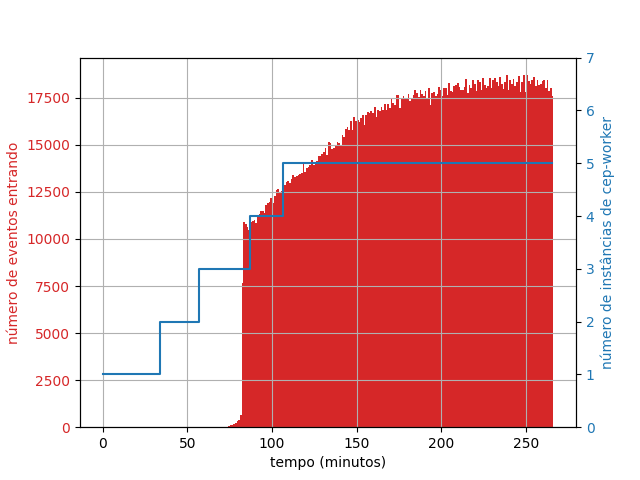
\includegraphics[width=\linewidth]{figuras/graphics/carga_e_workers_total8-dez-is.png}  
  \caption{Execução 3}
  \label{fig:cewt-8-dez-is}
\end{subfigure}
\begin{subfigure}{.5\textwidth}
  \centering
  % include second image
  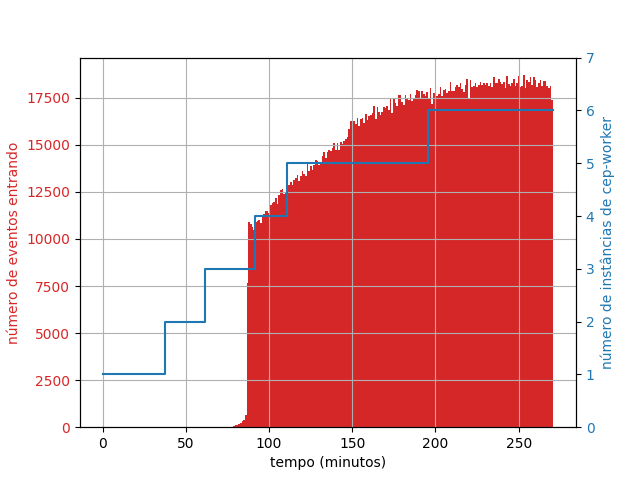
\includegraphics[width=\linewidth]{figuras/graphics/carga_e_workers_total9-dez-is.png}  
  \caption{Execução 4}
  \label{fig:cewt-9-dez-is}
\end{subfigure}
\begin{subfigure}{.5\textwidth}
  \centering
  % include second image
  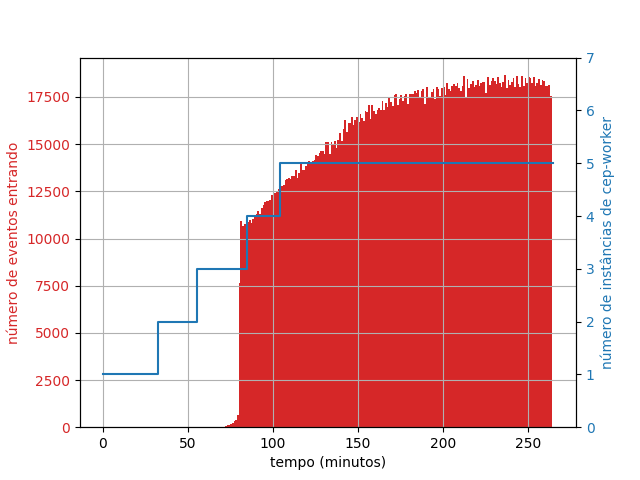
\includegraphics[width=\linewidth]{figuras/graphics/carga_e_workers_total10-dez-is.png}  
  \caption{Execução 5}
  \label{fig:cewt-10-dez-is}
\end{subfigure}
\caption{Número de eventos entrando no sistema (em vermelho) e número de instâncias de \texttt{CEP Worker} (em azul) em função do tempo nas execuções do experimento utilizando o algoritmo de balanceamento de carga por Similaridade de Entrada.}
%\todo[inline]{Os eixos y dos gráficos em azul (de número de workers) não estão iguais, induzindo a uma conclusão errada da comparação entre 2 execuções. Por exemplo, compare os gráficos das execuções 1 e 2. Parece que a execução 1 usa menos workers, porque a linha azul dela está mais tempo "abaixo" do contorno da carga de entrada (em vermelho) que a execução 2. Na execução 2, a linha azul está sempre acima do contorno da carga de entrada. Mas como o eixo y dessas duas execuções são diferentes, essa comparação "visual" não funciona. Fixe o eixo y azul em todos os gráficos desta figura e também na Figura 7.6. }
\label{fig:workers_and_events_IS}
\end{figure}
 
No experimento, escolheu-se fazer o cadastro de todos os tipos de eventos antes do início dos envios para que se pudesse distinguir melhor os efeitos do cadastro de novos eventos dos efeitos do aumento do número de eventos de entrada. As figuras \ref{fig:load_and_instances-time-SU}  e \ref{fig:load_and_instances-time-IS} mostram o crescimento do número de instâncias de \texttt{CEP Worker} pelo horário do dia da coleta do evento para todas as execuções. Elas melhor evidenciam a relação entre o número de instâncias e o aumento da carga de entrada no sistema.


\begin{figure}[h!]
\begin{subfigure}{.5\textwidth}
  \centering
  % include second image
  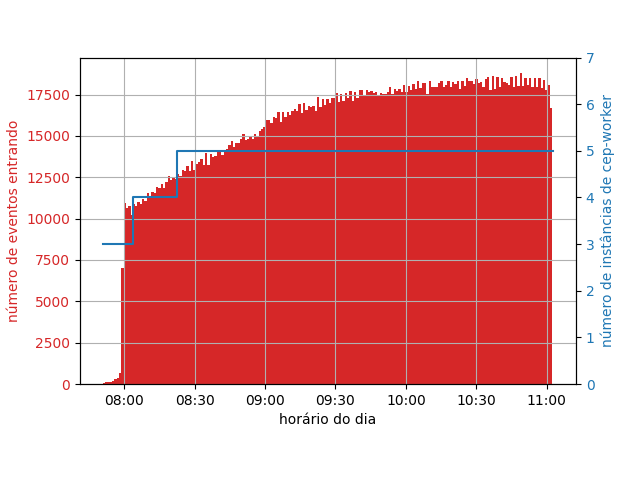
\includegraphics[width=\linewidth]{figuras/graphics/carga_e_workers_horario5-dez-su.png}  
  \caption{Execução 1}
  \label{fig:cewh-5-dez-su}
\end{subfigure}
\begin{subfigure}{.5\textwidth}
  \centering
  % include second image
  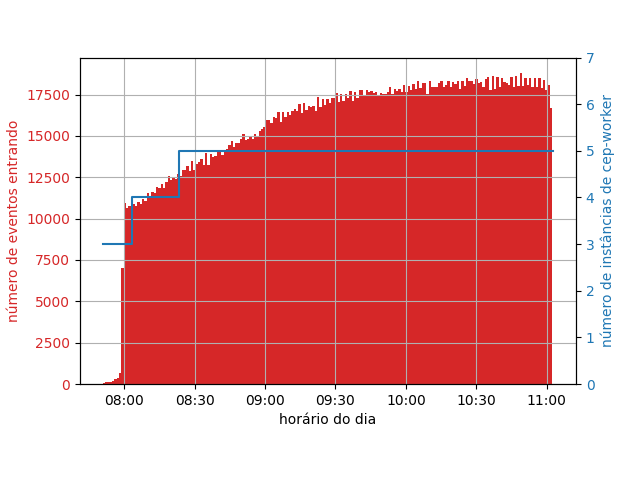
\includegraphics[width=\linewidth]{figuras/graphics/carga_e_workers_horario7-dez-su.png}  
  \caption{Execução 2}
  \label{fig:cewh-7-dez-su}
\end{subfigure}
\begin{subfigure}{.5\textwidth}
  \centering
  % include second image
  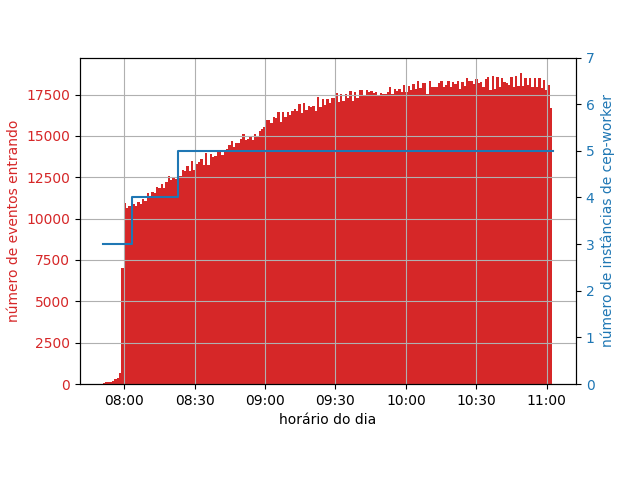
\includegraphics[width=\linewidth]{figuras/graphics/carga_e_workers_horario8-dez-su.png}  
  \caption{Execução 3}
  \label{fig:cewh-8-dez-su}
\end{subfigure}
\begin{subfigure}{.5\textwidth}
  \centering
  % include second image
  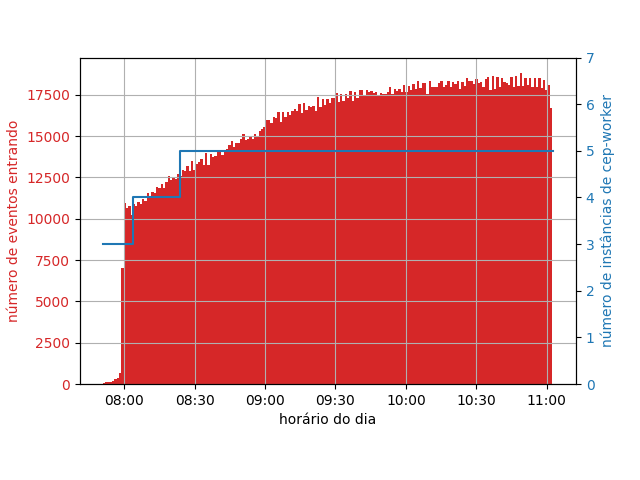
\includegraphics[width=\linewidth]{figuras/graphics/carga_e_workers_horario9-dez-su.png}  
  \caption{Execução 4}
  \label{fig:scewh-9-dez-su}
\end{subfigure}
\begin{subfigure}{.5\textwidth}
  \centering
  % include second image
  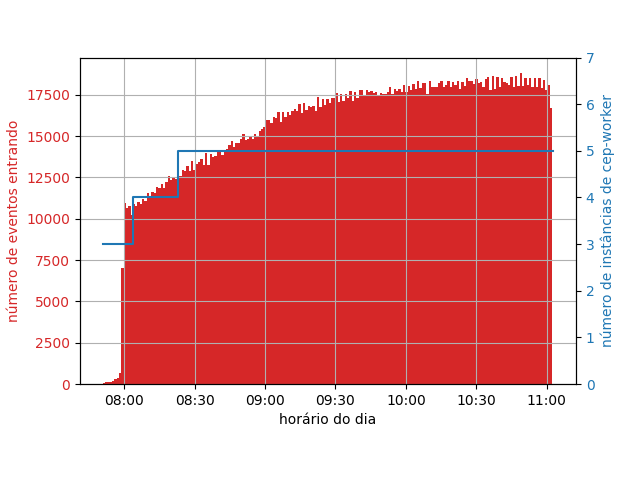
\includegraphics[width=\linewidth]{figuras/graphics/carga_e_workers_horario10-dez-su.png}  
  \caption{Execução 5}
  \label{fig:cewh-10-dez-su}
\end{subfigure}
\caption{Número de eventos entrando no sistema (em vermelho) e número de instâncias de \texttt{CEP Worker} (em azul) em função do horário do dia nas  execuções do experimento utilizando o algoritmo de balanceamento de carga por Uso de Estado.}
\label{fig:load_and_instances-time-SU}

%\todo[inline]{Fernando, esses gráficos da figura 7.5 não estão corretos. Todos eles são iguais, e não correspondem aos da Figura 7.3 (os quais eu tb acho que estão errados). :( }
\end{figure}



\begin{figure}[h!]
\begin{subfigure}{.5\textwidth}
  \centering
  % include second image
  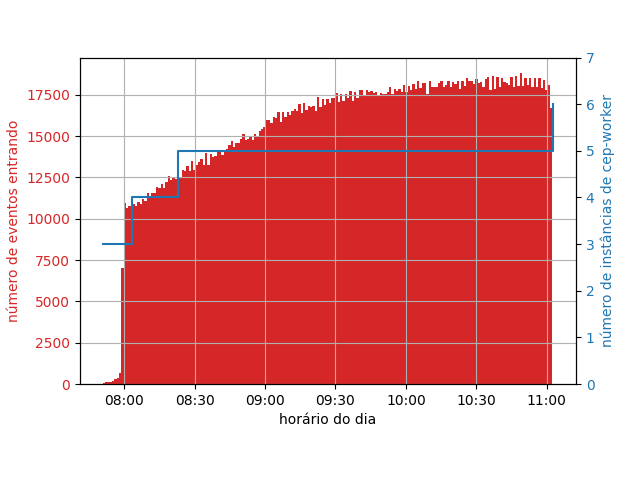
\includegraphics[width=\linewidth]{figuras/graphics/carga_e_workers_horario6-dez-is.png}  
  \caption{Execução 1}
  \label{fig:cewh-6-dez-is}
\end{subfigure}
\begin{subfigure}{.5\textwidth}
  \centering
  % include second image
  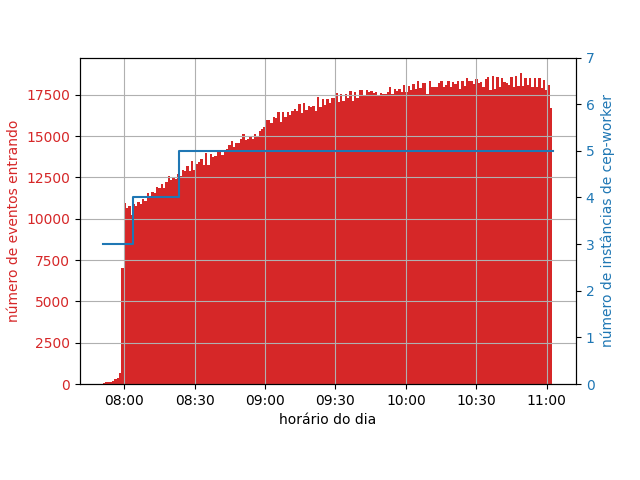
\includegraphics[width=\linewidth]{figuras/graphics/carga_e_workers_horario7-dez-is.png}  
  \caption{Execução 2}
  \label{fig:cewh-7-dez-is}
\end{subfigure}
\begin{subfigure}{.5\textwidth}
  \centering
  % include second image
  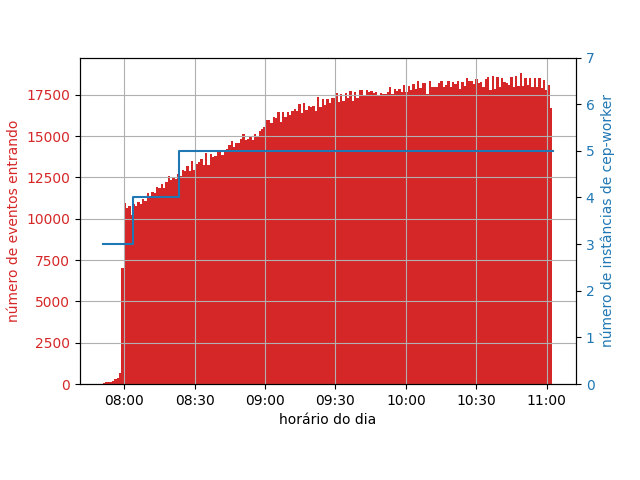
\includegraphics[width=\linewidth]{figuras/graphics/carga_e_workers_horario8-dez-is.png}  
  \caption{Execução 3}
  \label{fig:cewh-8-dez-is}
\end{subfigure}
\begin{subfigure}{.5\textwidth}
  \centering
  % include second image
  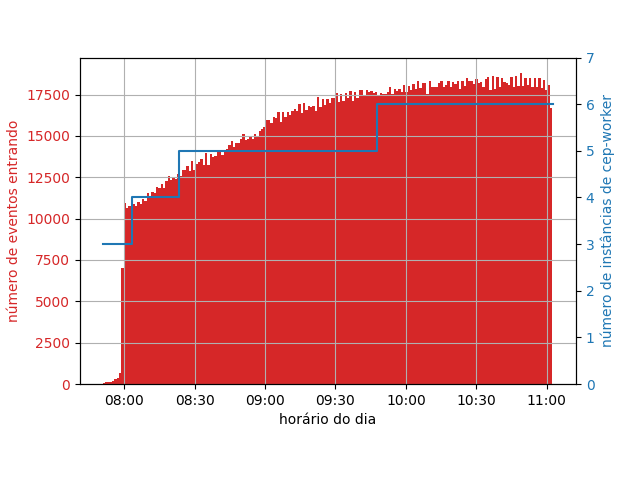
\includegraphics[width=\linewidth]{figuras/graphics/carga_e_workers_horario9-dez-is.png}  
  \caption{Execução 4}
  \label{fig:cewh-9-dez-is}
\end{subfigure}
\begin{subfigure}{.5\textwidth}
  \centering
  % include second image
  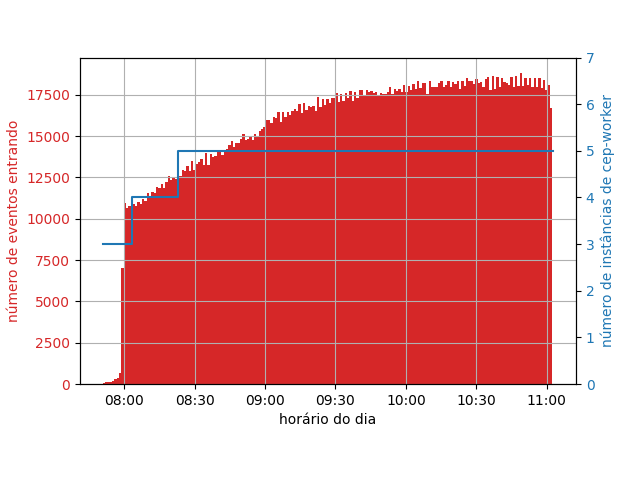
\includegraphics[width=\linewidth]{figuras/graphics/carga_e_workers_horario10-dez-is.png}  
  \caption{Execução 5}
  \label{fig:cewh-10-dez-is}
\end{subfigure}
\caption{Número de eventos entrando no sistema (vermelho)  e número de instâncias de \texttt{CEP Worker} (em azul) em função do horário do dia nas  execuções do experimento utilizando o algoritmo de balanceamento de carga por Similaridade de Entrada}
\label{fig:load_and_instances-time-IS}
%\todo[inline]{Assim como comentei para o gráfico 7.4, aqui você precisa fixar os eixos y azuis, para possibilitar a comparação visual entre as execuções. }
\end{figure}


%Das cinco repetições do experimento feitas para cada algoritmo de balanceamento de carga, 
Como mostra a Figura~\ref{fig:workers_and_events_SU}, em todas as cinco repetições do experimento usando o algoritmo de balanceamento por Uso de Estado, o número máximo de instâncias de \texttt{CEP Worker} em uso para lidar com a carga de eventos de entrada foi cinco. Já com o algoritmo de balanceamento por Similaridade de Entrada, duas das cinco repetições chegaram ao disparo de seis instâncias de \texttt{CEP Worker}, como mostrado na Figura~\ref{fig:workers_and_events_IS}. Em uma delas, a criação da sexta instância de \texttt{CEP Worker} ocorreu depois do final do envio de eventos primários. 
%As figuras \ref{fig:load_and_instances-time-SU-x} e \ref{fig:load_and_instances-time-IS-x} mostram um dos casos onde o número de instâncias não foi igual. Estas e todas as figuras das outras execuções podem ser encontradas em \autoref{ape:graphics}.




%No sistema \texttt{CEP Handler}, conforme descrito em \autoref{cap:arquitetura}, assim que o número de \texttt{CEP Workers} que estão aptos a receber realocação de tipos de eventos é menor que o número de \texttt{CEP Workers} que estão em sobrecarga e precisam realocar seus próprios tipos de eventos, um novo \texttt{CEP Workers} é instanciado. Então, assumindo que somente os três primeiros \texttt{CEP Workers}, que já tinham boa parte de sua memória em uso pelo simples cadastro de tipos de eventos atingissem a sobrecarga, o número máximo de instancias de \texttt{CEP Workers} atingido seria seis\todo{Esta última frase está confusa e a afirmação que ela tenta fazer é especulativa. Sugiro que o parágrafo todo seja removido do texto.}.


\section{Tempo de Uso de Recursos}
\label{sec:resource_usage_time}
%Na execução de um experimento auto-escalável, coletar os dados da variação do custo computacional entre uma execução e outra é fundamental para avaliar as diferenças que podem minimizar este custo. Durante os experimentos executados, considerando principalmente o custo de manter máquinas virtuais em funcionamento, a única variação que pode ser detectada é a diferença do número de instâncias de \texttt{cep worker} que estão ativas a cada momento. O propósito da coleta destes dados foi o de avaliar uma possível distinção entre o número de instâncias ativas em relação ao uso de cada um dos algoritmos de balanceamento de carga, descritos em \autoref{cap:arquitetura}.

%Em plataformas de nuvem, paga-se pelo uso dos recursos computacionais. A precificação leva em conta o tipo dos recursos alocados e o seu tempo de uso. 


Nas execuções do experimento de avaliação do \texttt{CEP Handler} na AWS, usou-se um só tipo de máquina virtual, o t3a.medium. Todos os microsserviços do experimento, listados no Capítulo \ref{cap:experimento}, foram instanciados nesse tipo de máquina virtual. Exceto pelo \texttt{CEP Worker}, utilizou-se somente uma instância para cada microsserviço. Portanto, a variação da quantidade de uso de recursos depende exclusivamente da instanciação de \texttt{CEP Workers} feita em cada execução.

A quantidade de máquinas virtuais alocadas dinamicamente para as instâncias de \texttt{CEP Workers} e os seus respectivos tempos de uso variaram de uma execução para outra, como mostrado na Seção~\ref{sec:auto_scalability}.
Mas o tempo total de uso de recursos variou relativamente pouco nas execuções.
A tabela \ref{Tab:time_and_avg} mostra o tempo de uso de recursos, em minutos, somado de todas as instâncias de \texttt{CEP Workers} para cada execução do experimento. As médias de tempo de uso de recursos dos dois algoritmos de balanceamento não apresentam uma diferença expressiva.
%Os valores de média de tempo de uso de recursos para o uso de cada um dos algoritmos não resultou em uma diferença expressiva em tempo de uso de máquinas virtuais.

%\begin{equation}
%    t = \frac{x - \mu}{\frac{s}{\sqrt{n}}} \\
%\end{equation}

%A partir do uso do teste T de Student para verificar a similaridade das medidas coletadas é possível afirmar que as duas distribuições não apresentam uma diferença significativa com um intervalo de confiança de 99\%.




%A média de tempo de uso de recursos das execuções usando o algoritmo de Similaridade de Entrada é maior que a média dos experimentos usando o algoritmo de Uso de Estado, no entanto os seus desvios padrão permitem dizer que as duas médias são similares.
%\todo[inline]{Fernando, creio que não é correto fazer a comparação das médias da forma como você fez, olhando para o DP. Seria preciso usar algum tipo de teste de hipóteses, como o teste t, para a comparação de amostras independentes (também chamadas de amostras não-pareadas). Veja exemplos em \url{http://www.leg.ufpr.br/lib/exe/fetch.php/disciplinas:ce001:bioestatistica_testes_t_para_comparacao_de_medias_de_dois.pdf} e \url{https://www.ime.usp.br/~sandoval/mae5755/comparacao_2medias\_\%20independentes.pdf}. Acho que não vai dar tempo de verificar isso até o dia 23. Mas anotei isso só pra vc lembrar de estudar sobre isso depois, para responder possíveis questionamentos da banca. }





\begin{table}[h!]
\centering
\caption{Tempo de uso de recursos em minutos de cada execução do experimento.}
\begin{tabular}{rr}
\multicolumn{1}{l}{\textbf{Balanceamento de Carga por}} & \multicolumn{1}{l}{\textbf{Balanceamento de Carga por}}  \\
\multicolumn{1}{l}{\textbf{Uso de Estado}} & \multicolumn{1}{l}{\textbf{Similaridade de Entrada}}  \\
 1.049,94 & 1.045,14  \\
1.041,69  & 1.054,98 \\
1.041,86  & 1.047,93 \\
1.042,23  & 1.052,84  \\
1.052,08  & 1.045,12  \\
\multicolumn{1}{l}{\textbf{Média}}& \multicolumn{1}{l}{\textbf{Média}} \\
1.045,56  & 1.049,2  \\
\multicolumn{1}{l}{\textbf{Desvio Padrão}} & \multicolumn{1}{l}{\textbf{Desvio Padrão}}  \\
 5,04 & 4,51                         
\end{tabular}
\label{Tab:time_and_avg}
\end{table}

%Na rede de processamento desenvolvida para o experimento, os tipos de eventos de detecção de agrupamento de ônibus de mesma linha (\textbf{busB}) foram definidos um por ônibus e utilizaram como fonte os tipos de evento de filtro de velocidade (\textbf{vi}), os quais foram definidos um por linha. Com isso, era possível agrupar todos os tipos de eventos de detecção de agrupamento de ônibus de uma mesma linha para a execução numa mesma instância de \texttt{CEP Worker}, minimizando a carga de entrada em cada instância no sistema. Como descrito no Capítulo \ref{cap:experimento}, dos 15.729 tipos de eventos criados, 14.121 eram de detecção de agrupamento de ônibus. Esse cenário, teoricamente, favoreceria o uso do algoritmo de balanceamento por Similaridade de Entrada. Contudo, isso não foi observado nos experimentos, já que os dois algoritmos resultaram em tempos médios de uso de recursos similares. \todo{Não se esqueça de corrigir a primeira parte deste parágrafo, que explica errado o que algoritmo faz. O alg não minimiza a carga de entrada de cada instância, ele tenta evitar a duplicação da transmissão de eventos para os nós. }
%, com o desempenho do algoritmo de Similaridade de Entrada minimamente pior que o do algoritmo de Uso de Estado.

%A diferença no número de instâncias criadas por cada algoritmo pode ser atribuída à diferença de velocidade de realocação dos tipos de eventos. O algoritmo de balanceamento por Uso de Estado seleciona os tipos de eventos cujo estado pode ser mais rapidamente reconstruído e, consequentemente, mais rapidamente realocado. Para a rede de processamento do experimento, selecionar para a realocação tipos de eventos que podem ser mais rapidamente realocados foi tão eficiente quanto selecionar para realocação tipos de eventos de forma que a carga de eventos de entrada em cada \texttt{CEP Worker} fosse minimizada\todo{O alg não minimiza carga de entrada!!!}. Logo, a velocidade de realocação de tipos de eventos foi um dos principais fatores para determinar o número de instâncias usados no experimento, pois em nenhum momento foi detectado que havia mais de duas instâncias em sobrecarga forte ao mesmo tempo\todo{Mas onde o leitor pode verificar isso que você está falando? Qual gráfico mostra que não havia mais do que duas instâncias em sobrecarga? os gráficos da figura \ref{fig:workers_and_events_SU} o numero de workers nunca passa de 5, enquanto os gráficos da figura \ref{fig:workers_and_events_IS} dois chegam a seis workers}. Caso essa situação fosse detectada, uma nova instância seria criada para lidar com as três\todo{por que três? pq as três primeiras que estavam cadastrando os tipos de eventos antes do envio dos eventos de entrada são as mais propensas a atingirem sobrecarga} em sobrecarga forte, como descrito na Seção \ref{sub-sec:cep-worker-func}\todo{essa seção citada diz que "quando o número de instâncias em sobrecarga forte é maior que o número de instâncias que não estão em nenhuma sobrecarga, uma nova instância de cep worker é requisitada". Então, a discussão depende tb de saber quantas instâncias não estão em sobrecarga. E isso você não menciona aqui. }. A realocação mais rápida de eventos pelo uso do algoritmo de balanceamento por Uso de Recursos minimizou o número de instâncias em sobrecarga forte em qualquer momento da execução. 
%\todo[inline]{Fernando, como conversamos por vídeo na sexta, essa explicação no parágrafo acima precisa ser revista, ou talvez retirada do texto mesmo. O raciocínio baseado na história das 3 instâncias em sobrecarga não está nada claro e não se apoia nos gráficos apresentados ao leitor. }
%O algoritmo de Similaridade de Entrada, utilizando-se do fato de vários destes tipos de eventos terem como fonte o mesmo tipo de evento de filtro de velocidade, tentou aloca-los no mesmo cep worker, atingindo um desempenho similar ao de algoritmo de Uso de Estado em relação ao custo computacional do experimento.

\section{Número de Eventos Detectados}
\label{sec:number_of_detected_events}


A Tabela \ref{Tab:events_total_and_avg} mostra o número de eventos detectados para cada uma das execuções do experimento, bem como a média e o desvio padrão para as execuções de cada um dos algoritmos de balanceamento de carga. A média do número de eventos detectados com o uso do algoritmo de balanceamento por uso de estado não foi expressivamente diferente da média de eventos detectados com o uso do algoritmo de balanceamento por Similaridade de Entrada. %Considerando a média e o intervalo de desvio padrão, eles detectaram um número de eventos similar\todo{Aqui vale o mesmo comentário que fiz na comparação de médias anterior: o mais correto seria usar um teste estatístico}.
Embora isso não possa ser visto na tabela, foi verificado que a diferença entre o número de eventos primários que foram enviados como entrada e depois coletados na saída do sistema em cada experimento foi nula. Isso sugere que as diferenças no número de eventos detectados mostradas na Tabela \ref{Tab:events_total_and_avg} não são devido a problemas de conexão. 

%\todo[inline]{É preciso ter consistência. O capítulo quase todo referencia os algoritmos pelo nome (inclusive nas figuras e tabelas). Mas aqui (e em alguns outros poucos lugares) você referenciou pelo número. Use somente o nome em todo lugar, ou use somente o número em todo lugar. Mas não misture os dois estilos de referência aos algoritmos, senão confunde o leitor.}
%\todo[inline]{Ao longo do capítulo, a uma outra inconsistência relacionada aos algs. Em algumas figuras e tabelas, a ordem de apresentação dos resultados é primeiro para o Alg por Uso de Estado e depois para o Similaridade. Em outras, a ordem é a inversa. Isso também confunde bastante. É preciso adotar uma só ordem.}


\begin{table}[h!]
\centering
\caption{Número de eventos detectados em cada execução do experimento.}
\begin{tabular}{rr}
\multicolumn{1}{l}{\textbf{Balanceamento de Carga por}} & \multicolumn{1}{l}{\textbf{Balanceamento de Carga por}}  \\
\multicolumn{1}{l}{\textbf{Uso de Estado}} & \multicolumn{1}{l}{\textbf{Similaridade de Entrada}}  \\
     1.703.200   &    1.706.853     \\
           1.705.963    & 1.707.100 \\
       1.704.298    &   1.703.770   \\
        1.709.012    &  1.703.887  \\
            1.707.569  &  1.704.115 \\
\multicolumn{1}{l}{\textbf{Média}}& \multicolumn{1}{l}{\textbf{Média}}\\
       1.706.008,4   &  1.705.145  \\
\multicolumn{1}{l}{\textbf{Desvio Padrão}}& \multicolumn{1}{l}{\textbf{Desvio Padrão}} \\
 2.359,65   &  1.678,79 
\end{tabular}
\label{Tab:events_total_and_avg}
\end{table}
%\todo[inline]{Formate mais uniformemente as tabelas desta seção. Destaque os nomes com negritos, para melhorar a legibilidade. Coloque pontos para separar os milhares dos números.}

A principal causa das diferenças no número de eventos detectados fica mais clara ao olhar para os resultados separados por categoria de tipo de evento para cada execução do experimento. As tabelas \ref{Tab:events_SU_and_avg} e \ref{Tab:events_IS_and_avg} mostram que não há diferença no número de eventos coletados para tipos de evento de cálculo de velocidade instantânea e de filtro de velocidade. A diferença só é expressa nos eventos obtidos a partir de tipos de eventos que utilizam janelas temporais. O uso de janelas temporais para os operadores de agregação nesses tipos de eventos faz com que o número total de eventos gerados por eles seja impactado pela variação de latência dos seus eventos de entrada. Como a distribuição das latências ao longo do tempo muda de uma execução do experimento para outra (como será mostrado na Seção~\ref{sec:latency}), isso causa as discrepâncias no número de eventos gerados por esses tipos de eventos em diferentes execuções.
%\todo[inline]{Essa explicação dada na parte final do parágrafo acima não parece correta. Não é a "distribuição de latências desigual ao longo da execução" de um experimento que causa a diferença de qtde de detecções em duas execuções diferentes. O que causa a diferença na qtde é a diferença das distribuições das latências das execuções, certo? }





\begin{table}[h!]
\centering
\caption{Número de eventos detectados por categoria de tipo de evento em cada execução do experimento com o algoritmo de balanceamento por Uso de Estado.}
\begin{tabular}{lrrrrr}
          & \multicolumn{1}{l}{\textbf{vf}} & \multicolumn{1}{l}{\textbf{vi}} & \multicolumn{1}{l}{\textbf{vel}} & \multicolumn{1}{l}{\textbf{BusB}} & \multicolumn{1}{l}{\textbf{corr}}  \\
  & 1.434.615 & 80.528 & 26.613  & 138.452 & 26.645   \\
  & 1.434.615 & 80.530 & 26.608 & 138.667  & 26.680      \\
  & 1.434.615 & 80.529   & 26.541    & 135.752    & 26.333                     \\
  & 1.434.615 & 80.529   & 26.534    & 135.860    & 26.349                     \\
 & 1.434.615 & 80.528   & 26.563    & 136.007    & 26.402                     \\
\textbf{Média}      & 1.434.615 & 80.528,8 & 26.571,8  & 136.947,6  & 26.481,8                   \\
\textbf{Desvio Padrão}   & 0       & 0,8367      & 36,95        & 1476,19         & 167,38         
\end{tabular}
\label{Tab:events_SU_and_avg}
\end{table}


\begin{table}[h!]
\centering
\caption{Número de eventos detectados por categoria de tipo de evento em cada execução do experimento com o algoritmo de balanceamento por Similaridade de Entrada.}
\begin{tabular}{lrrrrr}
          & \multicolumn{1}{l}{\textbf{vf}} & \multicolumn{1}{l}{\textbf{vi}} & \multicolumn{1}{l}{\textbf{vel}} & \multicolumn{1}{l}{\textbf{BusB}} & \multicolumn{1}{l}{\textbf{corr}}  \\
  & 1.434.615 & 80.529   & 26.522    & 135.246    & 26.288                     \\
  & 1.434.615 & 80.528   & 26.585    & 137.671    & 26.564                     \\
  & 1.434.615 & 80.528   & 26.537    & 136.227    & 26.391                     \\
  & 1.434.615 & 80.529   & 26.718    & 140.277    & 26.873                     \\
 & 1.434.615 & 80.530   & 26.644    & 139.071    & 26.709                     \\
\textbf{Média}          & 1.434.615 & 80.528,8 & 26.601,2  & 137.698,4  & 26.565                     \\
\textbf{Desvio Padrão}           & 0       & 0,8367      & 80,83        & 2.044,09         & 235,91         
\end{tabular}
\label{Tab:events_IS_and_avg}
\end{table}


Ao observar, como exemplo de tipo de evento que não utiliza janela temporal, a diferença entre o valor máximo e mínimo do número de eventos dos tipos de filtro de velocidade (\textbf{vi}), verifica-se que foram coletados no máximo 80.530 e no mínimo 80.528 eventos, sendo a diferença de apenas 2 eventos, ou seja, de 0,00002\%. Isso é um indício de que não houve perda significativa de eventos no sistema por parte de transmissão entre instâncias de \texttt{CEP Worker} ou por outros mecanismos do experimento.



%------------------------------------------------------






%Nós escolhemos utilizar a mediana, pois observamos alguns eventos específicos que apresentavam latências muito maiores, levando a média a níveis fora do padrão de sistemas em tempo real


\section{Vazão}
\label{sec:vazao}

A vazão do sistema pode ser definida como a quantidade de dados transmitidos por intervalo de tempo~\citep{bukh1992art}. Neste trabalho, a vazão do \textit{CEP Handler} é definida como a quantidade de eventos por minuto transmitidos pelas instâncias de \texttt{CEP Worker} para o sistema de mensageria, para serem utilizados como entrada na detecção de outros tipos de eventos ou para o consumo do usuário final. %\todo{aqui neste frase você misturou uma definição de vazão vinda da ref bibliográfica e a sua definição de vazão no seu sistema. você tem que separar essas duas definições em duas frases diferentes: primeiro a definição clássica, depois a sua definição. A vazão é uma quantidade por unidade de tempo; você precisa deixar isso claro na definição, precisa dizer qual é a unidade de tempo da sua vazão (minuto)}. 
As figuras \ref{fig:histogram_full_IS} e \ref{fig:histogram_full_SU} mostram a vazão do sistema ao longo de uma execução do experimento para cada algoritmo de balanceamento. Na figuras, pode-se observar que existe um crescimento da vazão ao longo do tempo similar ao da carga de entrada. 

 \afterpage{\clearpage}

\begin{figure}[h!]
\begin{subfigure}{.5\textwidth}
  \centering
  % include second image
  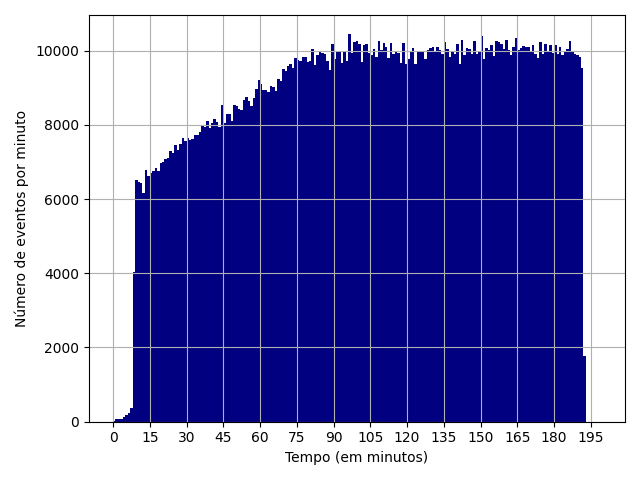
\includegraphics[width=.8\linewidth]{figuras/graphics/histogram_vazao_5-dez-su.png}  
  \caption{Execução 1}
  \label{fig:histv-5-dez-su}
\end{subfigure}
\begin{subfigure}{.5\textwidth}
  \centering
  % include second image
  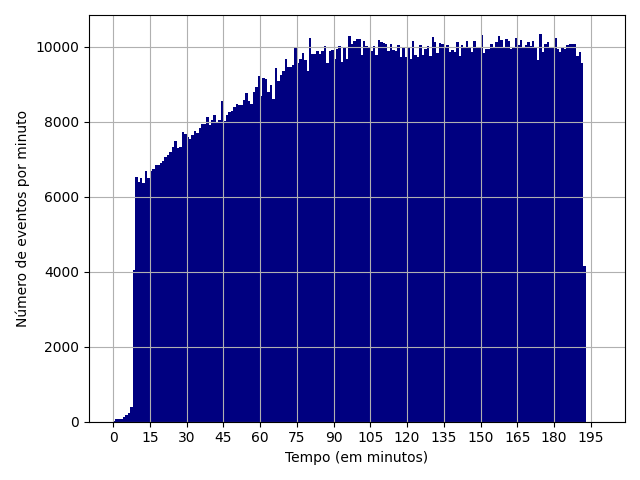
\includegraphics[width=.8\linewidth]{figuras/graphics/histogram_vazao_7-dez-su.png}  
  \caption{Execução 2}
  \label{fig:histv-7-dez-su}
\end{subfigure}
\begin{subfigure}{.5\textwidth}
  \centering
  % include second image
  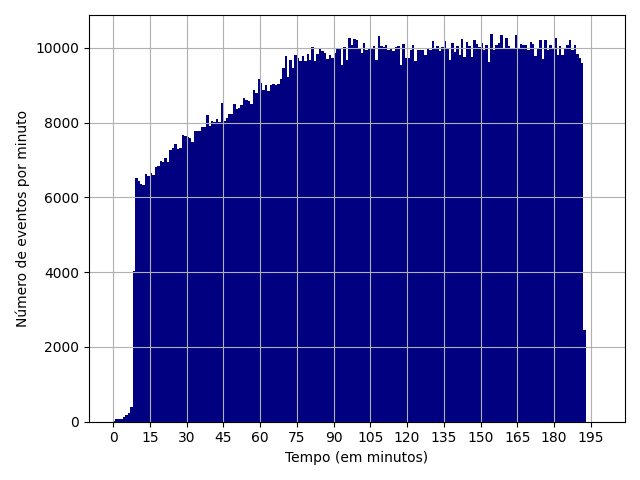
\includegraphics[width=.8\linewidth]{figuras/graphics/histogram_vazao_8-dez-su.png} 
  \caption{Execução 3}
  \label{fig:histv-8-dez-su}
\end{subfigure}
\begin{subfigure}{.5\textwidth}
  \centering
  % include second image
  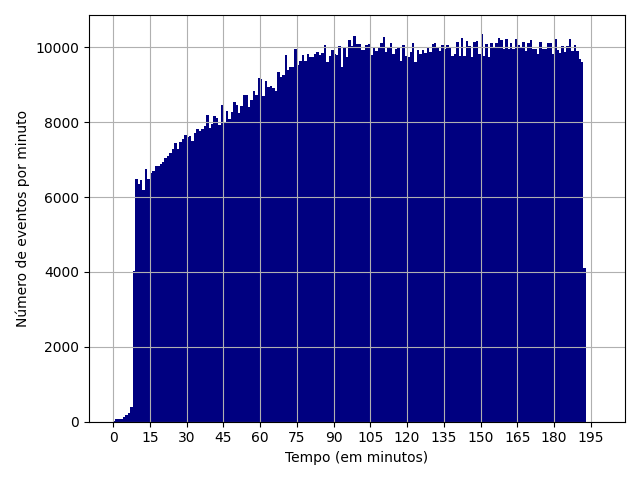
\includegraphics[width=.8\linewidth]{figuras/graphics/histogram_vazao_9-dez-su.png}  
  \caption{Execução 4}
  \label{fig:histv-9-dez-su}
\end{subfigure}
\begin{subfigure}{.5\textwidth}
  \centering
  % include second image
  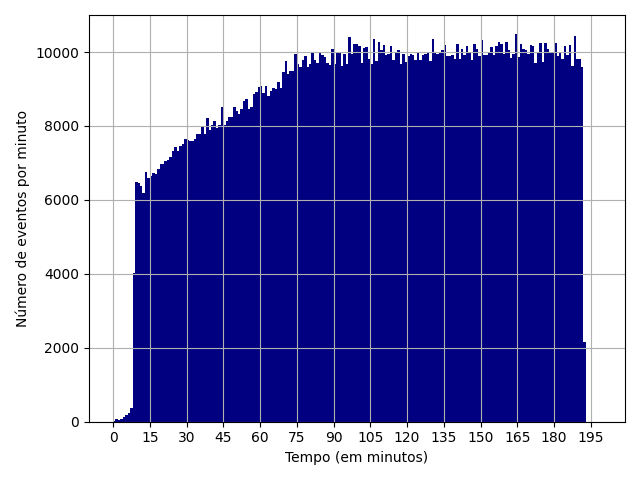
\includegraphics[width=.8\linewidth]{figuras/graphics/histogram_vazao_10-dez-su.png}  
  \caption{Execução 5}
  \label{fig:histv-10-dez-su}
\end{subfigure}
\caption{Vazão de eventos detectados pelo sistema nas  execuções do experimento utilizando o algoritmo de de balanceamento por Uso de Estado.}
\label{fig:histogram_full_SU}
%\todo[inline]{Verificar se vai usar no capítulo nome do alg ou número do alg., para corrigir a legenda se necessário.}
\end{figure}

 \afterpage{\clearpage}

\begin{figure}[h!]
\begin{subfigure}{.5\textwidth}
  \centering
  % include second image
  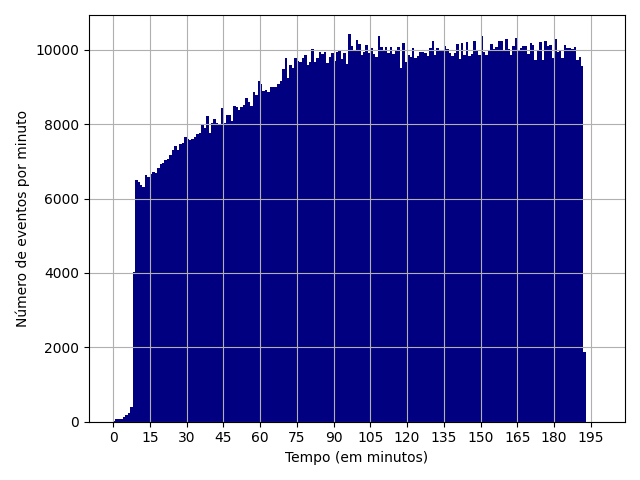
\includegraphics[width=\linewidth]{figuras/graphics/histogram_vazao_6-dez-is.png}  
  \caption{Execução 1}
  \label{fig:histv-6-dez-is}
\end{subfigure}
\begin{subfigure}{.5\textwidth}
  \centering
  % include second image
  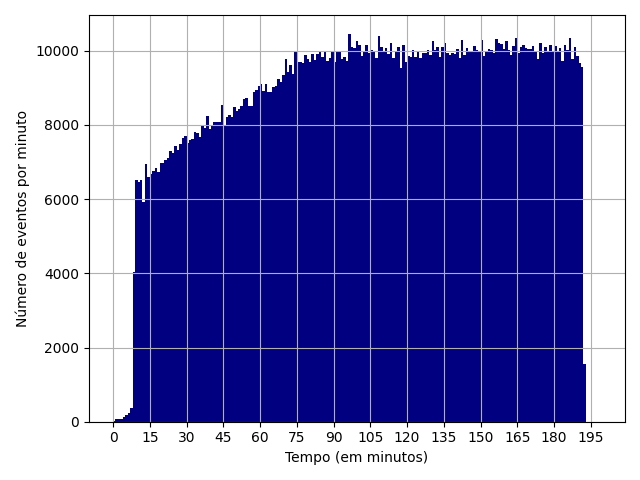
\includegraphics[width=\linewidth]{figuras/graphics/histogram_vazao_7-dez-is.png}  
  \caption{Execução 2}
  \label{fig:histv-7-dez-is}
\end{subfigure}
\begin{subfigure}{.5\textwidth}
  \centering
  % include second image
  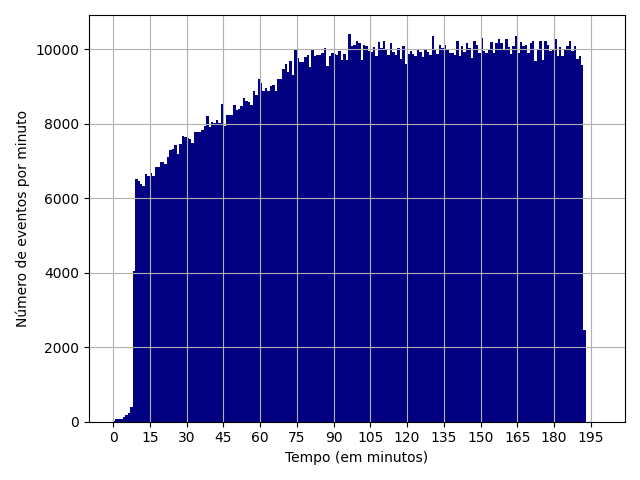
\includegraphics[width=\linewidth]{figuras/graphics/histogram_vazao_8-dez-is.png} 
  \caption{Execução 3}
  \label{fig:histv-8-dez-is}
\end{subfigure}
\begin{subfigure}{.5\textwidth}
  \centering
  % include second image
  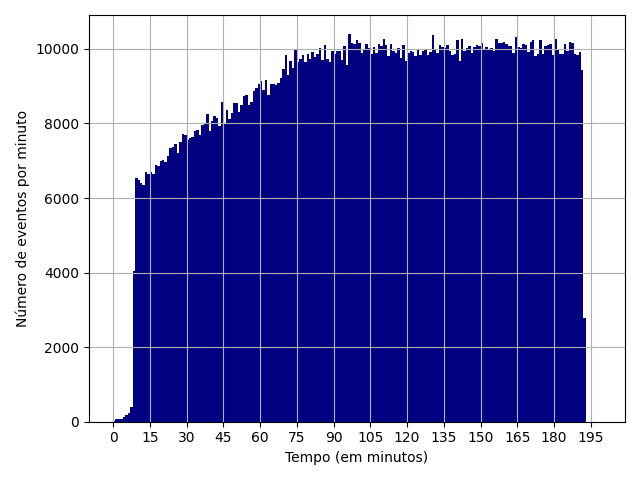
\includegraphics[width=\linewidth]{figuras/graphics/histogram_vazao_9-dez-is.png}  
  \caption{Execução 4}
  \label{fig:histv-9-dez-is}
\end{subfigure}
\begin{subfigure}{.5\textwidth}
  \centering
  % include second image
  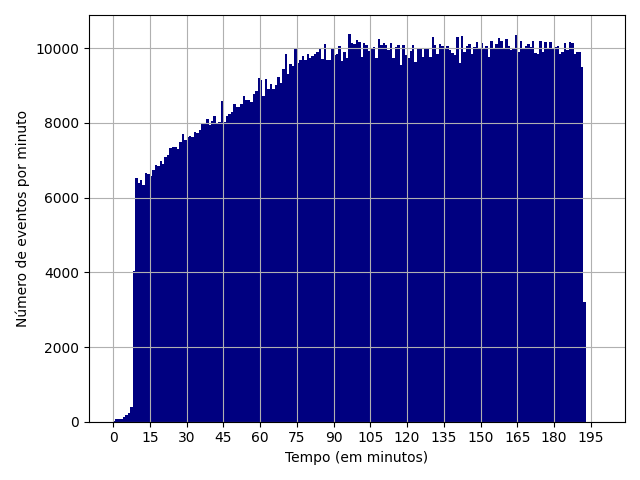
\includegraphics[width=\linewidth]{figuras/graphics/histogram_vazao_10-dez-is.png}  
  \caption{Execução 5}
  \label{fig:histv-10-dez-is}
\end{subfigure}
\caption{Vazão de eventos detectados pelo sistema nas execuções do experimento utilizando o algoritmo de balanceamento por Similaridade de Entrada.}
%\todo[inline]{Verificar se vai usar no capítulo nome do alg ou número do alg., para corrigir a legenda se necessário.}
\label{fig:histogram_full_IS}
\end{figure}


%A vazão do sistema, ou seja, o número de eventos que foram transmitidos por intervalo de tempo, foi crescente durante o experimento, seguindo a curva de eventos que entravam no sistema. 
As figuras que mostram a variação de vazão de todas as execuções do experimento podem ser encontradas no Apêndice \ref{ape:graphics}. Comparando os gráficos das execuções que usam o algoritmo de balanceamento de carga por Uso de Estado com os do algoritmo por Similaridade de Entrada, não é possível notar uma diferença significativa nas vazões do sistema, para qualquer sub-intervalo de tempo do experimento. A pequena variação observada na vazão do sistema pode se originar da variação de latência ao longo do tempo dos eventos de entrada para cada tipo de evento, principalmente para os tipos de eventos que usam janelas de tempo para a detecção. Esse é o caso dos tipos de evento de detecção de agrupamento de ônibus, que são maioria na rede de processamento de eventos do cenário do experimento, como já discutido na Seção \ref{sec:number_of_detected_events}.
%, o número geral de eventos detectados e a vazão do sistema são afetados pela latência do sistema.



\newpage
\section{Latência}
\label{sec:latency}



%As figuras \ref{fig:boxplot_vf_is_1} e \ref{fig:boxplot_vf_su_1} diagramas de caixas que mostram a variação das latências dentro de intervalos de cinco minutos, para o tipo de evento de cálculo de velocidade instantânea em uma execução de cada um dos dois algoritmos de balanceamento de carga. Os gráficos mostram que a latência mediana cresce desde o início da execução do experimento e se estabiliza no patamar de sessenta milissegundos. Este resultado é verificado para todas as outras execuções, cujos gráficos se encontram no \ref{ape:graphics}.
%\todo[inline]{Aqui, há aquele mesmo problema que apontei anteriormente: não faz sentido colocar esse par de execuções das figuras 7.9 e 7.10 lado a lado, para contrastar os desempenhos dos dois algs. Seria melhor criar uma figura com 5 subfigures das execuções para cada algoritmo. Ao invés de mostras esses graficos para o operador vi, acho que seria mais interessante mostrar para o busB, já que esse tipo de evento é maioria no sistema. Depois da inclusão desses gráficos, é precio ajustar o texto do parágrafo acima.}




Em um sistema que lida com dados em tempo real, a latência da transmissão de eventos pelo sistema é a principal métrica de análise do desempenho. Para medir a latência no \texttt{CEP Handler}, foi usado o método descrito na Seção  \ref{sec:experiment_architecture}. Uma marca temporal foi gerada no momento em que o evento primário foi enviado do microsserviço do experimento para ser consumido pelas instâncias de \texttt{CEP Workers}. Outra marca temporal foi gerada quando o evento foi armazenado no banco de dados chave-valor, depois de sua detecção pelo sistema. A latência foi tomada como a diferença entre esses dois valores. O tempo utilizado para os intervalos no eixo x dos gráficos de latência vêm da marca temporal de quando o evento foi armazenado, depois da detecção. 

Cada uma das figuras de \ref{fig:boxplot_vf_agg_1} a \ref{fig:boxplot_BusB_agg} mostram as latências das execuções de uma categoria de tipos de evento, separadas por algoritmo de balanceamento de carga. Diagramas de caixa foram usados para representar a variação de latência das execuções. Cada caixa mostra o primeiro quartil, a mediana e o terceiro quartil das latências de uma execução.  As linhas que se estendem a partir de uma caixa indicam a variabilidade fora do quartil superior e do quartil inferior.  % - \todo{Só para te avisar: expliquei aqui como ler os diagramas de caixa.}

%A latência observada nos experimentos não foi afetada significativamente pela escolha de algoritmo de balanceamento de carga. 
%Observando as figuras, é possível ver que o intervalo de latências foi similar entre todas as execuções e entre todos os tipos de eventos, ou seja, não houve uma diferença expressiva entre o uso de um algoritmo ou outro.
%\todo[inline]{Eu continuo achando que não podemos afirmar que as latências foram similares, como vc fez no parag acima. De qualquer forma, não há a necessidade de afirmar isso, certo? Para mim, já seria suficiente dizer que a latência da grande maioria dos eventos detectados ( > 75\%) fica abaixo de 100ms, como os gráficos mostram. Tentei incorporar isso ao parágrafo abaixo, veja se está de acordo.}
%\todo{Essa última frase está estranha. Olhando os gráficos, parece que o algoritmo por Uso de Estado tem latências ligeiramente maiores. }.

  Como mostram os diagramas de caixa, o sistema mostrou um bom desempenho em relação à latência para todos os tipos de eventos da rede de processamento. A grande maioria das latências fica abaixo de cem milissegundos, mesmo para os eventos que estão no final da rede de processamento e que dependem da detecção de toda uma cadeia de eventos. 
  
  Essas latências atendem de forma satisfatória os requisitos de processamento em tempo real dos dados da aplicação considerada no experimento -- o monitoramento de tráfego de ônibus de uma grande cidade. Essa rapidez na detecção e notificação dos eventos habilita a administração pública e as empresas que cuidam da gestão do transporte por ônibus a tomar ações para a resolução de problemas de tráfego em tempo oportuno. 
  
%o objetivo proposto para a detecção em tempo real neste trabalho, que é a detecção de acontecimentos fora do padrão em cidades inteligentes para a notificação da administração pública e empresas interessadas. 

%Nessa aplicação, para eventos que estão no final da rede de processamento de eventos e que dependem da detecção de toda uma cadeia de eventos, uma latência de menos de 100 milissegundos  é pequena o suficiente para notificar os interessados e disparar suas respectivas respostas . % citar aqui trabalhos relacionados que apresentam latencias similares - trabalhos relacionados não mencionam latencia.


%\todo[inline]{Nas últimas figuras, você apresenta primeiro os resultados do alg de similaridade e depois o de uso. Mas nas figuras anteriores, a ordem usada foi a inversa. Padronize a ordem deles nas figuras do capítulo todo, para não confundir o leitor.}



%Os gráficos de \textit{boxplot}  mostram a evolução da latência por tempo, ao longo de uma execução de um experimento, com a figura \ref{fig:boxplot_vf_su_1} representando uma execução utilizado o algoritmo de balanceamento de carga de Uso de Estado, enquanto que a figura \ref{fig:boxplot_vf_is_1} representa uma execução utilizando o algoritmo de balanceamento de carga de Similaridade de Entrada. Estas e as outras figuras mostrando a latência por tempo para cada execução podem ser encontradas no apêndice \ref{ape:graphics} .

%Os dados de cada um dos tipos de eventos com definições similares para linhas ou corredores distintos foram agrupados no mesmo gráfico, sendo que os dois gráficos das figuras \ref{fig:boxplot_vf_is_1} e \ref{fig:boxplot_vf_su_1} representam as latências do tipo de evento de cálculo de velocidade instantânea.
 \afterpage{\clearpage}

\begin{figure}[ht]
\centering
 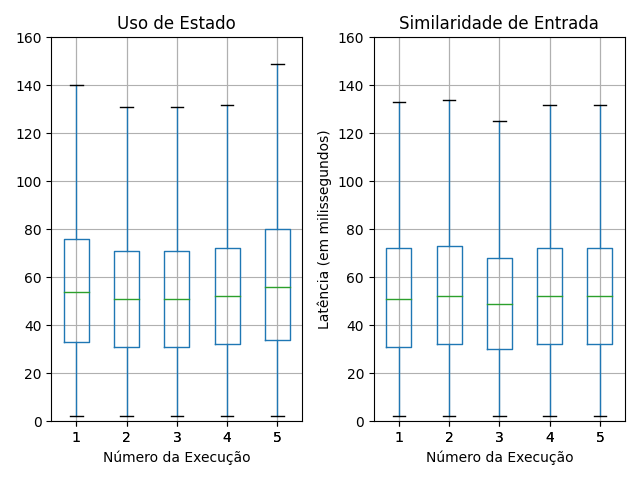
\includegraphics[width=0.7\textwidth]{figuras/graphics/boxplot_agg_vf.png}
 \caption{Latência para velocidade instantânea nas execuções do experimento para cada algoritmo de balanceamento de carga.}
 \label{fig:boxplot_vf_agg_1}
\end{figure}

\afterpage{\clearpage}

\begin{figure}[ht]
  \centering
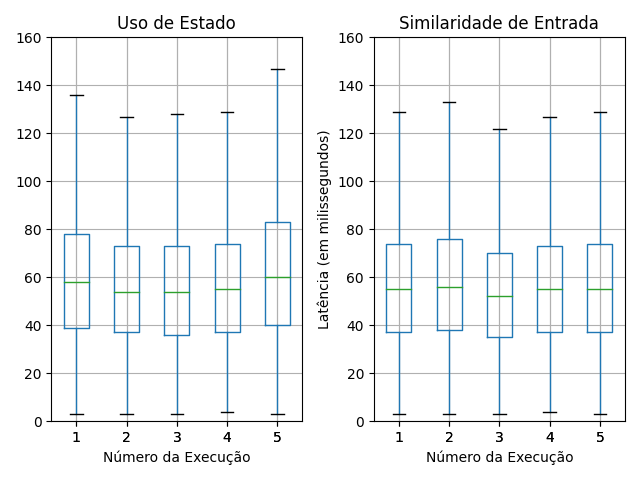
\includegraphics[width=0.7\textwidth]{figuras/graphics/boxplot_agg_vi.png}
\caption{Latência para filtro de velocidade nas execuções do experimento para cada algoritmo de balanceamento de carga.}
\label{fig:boxplot_vi_agg_1}
\end{figure}

\begin{figure}[ht]
  \centering
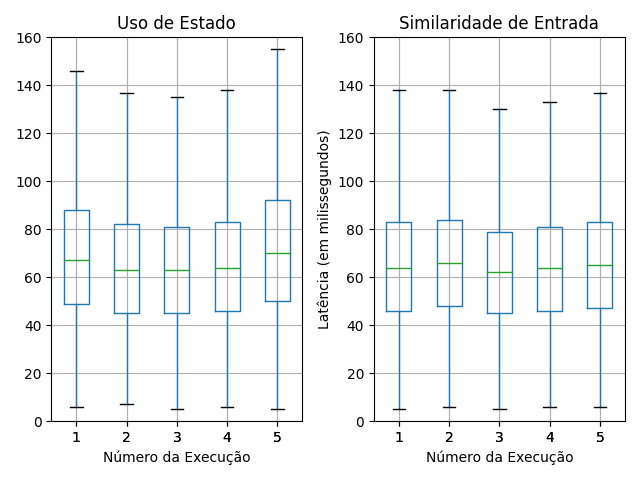
\includegraphics[width=0.7\textwidth]{figuras/graphics/boxplot_agg_vel.png}
\caption{Latência para velocidade média de ônibus nos corredores nas execuções do experimento para cada algoritmo de balanceamento de carga.}
\label{fig:boxplot_vel_agg}
\end{figure}

\begin{figure}[ht]
\centering
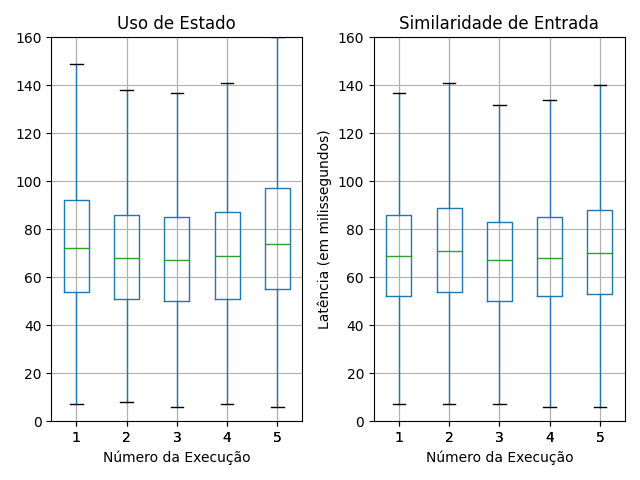
\includegraphics[width=0.7\textwidth]{figuras/graphics/boxplot_agg_corr.png}
 \caption{Latência para velocidade média de cada corredor nas execuções do experimento para cada algoritmo de balanceamento de carga.}
 \label{fig:boxplot_corr_agg}
\end{figure}


\afterpage{\clearpage}

\begin{figure}[ht]

  \centering
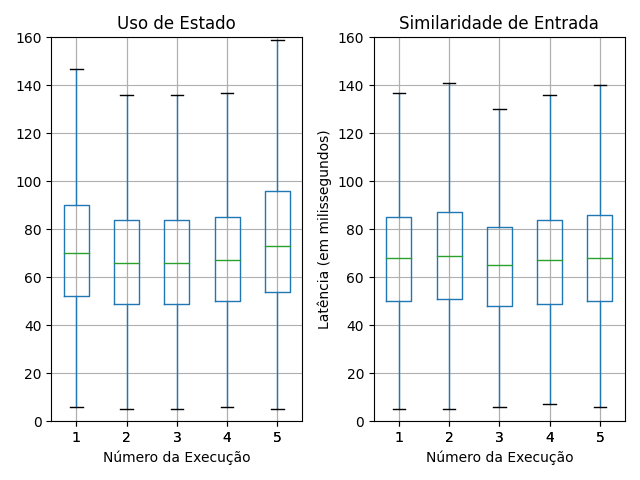
\includegraphics[width=0.7\textwidth]{figuras/graphics/boxplot_agg_BusB.png}
\caption{Latência para detecção de agrupamento de ônibus nas execuções do experimento para cada algoritmo de balanceamento de carga.}
\label{fig:boxplot_BusB_agg}

\end{figure}

  %\todo[inline]{Incluir "Número da execução" como rótulo no eixo x  desses últimos gráficos.}


%Comparando os resultados para os mesmos tipos de eventos é possível observar que a mediana da latência ficou abaixo de 200 ms em todos os casos. A latência cresce desde o inicio do experimento até chegar a um patamar estável. Esse crescimento segue a estabilização do número de instâncias de cep workers e o número de eventos entrando no sistema. 


%As figuras \textbf{XXXXX} mostram uma comparação das medianas totais de cada experimento, para ambos os algoritmos de balanceamento de carga. Como é possível observar, não há uma diferença significativa entre os valores de latência das execuções. Todas obtiveram um desempenho similar no experimento.



\section{Conclusão}


A análise dos resultados dos experimentos em relação a latência, vazão, número de eventos detectados e tempo de uso de recursos indica que os dois algoritmos de balanceamento de carga obtiveram resultados próximos e permitiram o sistema satisfazer o requisito de auto-escalabilidade. 

Os tipos de eventos utilizados no experimento foram escolhidos para a detecção de um número suficiente de respostas, para a obtenção de mais dados de latência de forma que ainda detectassem ocorrências importantes para a administração da frota de ônibus municipal. O terceiro quartil das latências medidas durante todas as execuções ficou sempre abaixo de cem milissegundos, para todas as categorias de tipos de eventos e considerando o uso de ambos os algoritmos de balanceamento de carga. Para servir os serviços urbanos de transporte, como os do cenário experimental utilizado neste trabalho, essa latência não impacta significativamente o intervalo de tempo entre a  ocorrência de um problema nas vias de circulação urbanas e a chegada das autoridades para resolução do problema detectado. 


A vazão e o número de eventos detectados pelo experimento são dependentes da latência no caso de tipos de eventos com janela temporal, como discutido na Seção \ref{sec:vazao}, pois para agrupar os eventos em janelas, os horários de chegada dos eventos no \texttt{CEP Worker} são usados%\todo{Explicação estranha. As suas janelas são deslizantes, então um mesmo evento pode entrar nas agregações de vários intervalos. Que tal trocar por: ", pois para agrupar os eventos em janelas, os horários de chegada dos eventos no \texttt{CEP Worker} são usados"}
. Para os eventos de outros tipos, a vazão e o número de eventos detectados não se alteram de uma execução para outra.

%ou seja, só dependem da velocidade de emissão de eventos pelo produtor de eventos em uso .\todo{O que vem depois do "ou seja",  está errado. Primeiro porque não diz a mesma coisa dita na primeira parte da frase. Segundo porque, se não tem janela, a qtde detectada NÃO muda com a velocidade de entrada. } 

A o tempo médio de uso de recursos computacionais pelas instâncias de \texttt{CEP Worker} em cada execução do experimento não foi expressivamente diferente para o dois algoritmos de balanceamento de carga, sendo de  $1.049,2 \pm 4,51$ minutos para o Algoritmo de balanceamento por Similaridade de Entrada e $1.045,56 \pm 5,04$ minutos para o algoritmo de balanceamento por Uso de Estado. Portanto, no cenário usado no experimento, o uso de um algoritmo de balanceamento de carga não foi expressivamente mais eficaz que o outro na economia de recursos computacionais. Como discutido na Seção \ref{sec:resource_usage_time}, uma possível explicação é que a alta velocidade de realocação dos tipos de eventos é um fator importante para minimizar o intervalo de tempo que cada instância se mantêm em sobrecarga. Como todas as execuções do experimento que utilizaram o algoritmo de balanceamento de carga por uso de estado chegaram a um máximo de cinco instâncias ativas ao mesmo tempo, de acordo com o mecanismo de requisição de novas instâncias descrito na Seção \ref{sec:cepworker}, em nenhum momento três das cinco instâncias estavam em sobrecarga forte ao mesmo tempo, ou seja, o uso do algoritmo propiciou um máximo de duas instâncias em sobrecarga forte em qualquer momento ao longo do experimento

Em comparação, o algoritmo de balanceamento de carga por Similaridade de Entrada buscava minimizar o número de eventos entrando em cada instância em sobrecarga forte, como descrito na Seção \ref{sec:cepworker}. As execuções do experimento com esse algoritmo não buscavam necessariamente selecionar os tipos de eventos que seriam mais rapidamente realocados e levaram a um máximo de seis instâncias de \texttt{CEP Worker} ativas em alguns casos. No entanto, a diferença em tempo de uso das instâncias médio foi similar entre o uso de um algoritmo de balanceamento de carga e o outro.

\todo[inline]{Conforme já conversamos, essa explicação é incorreta, porque o alg não faz essa minimização. O que ele faz é, na escolha do tipo de evento para realocação, privilegiar os tipos que não causam ou que causam menos a duplicação de fluxos de entrada}.  

%\todo[inline]{Ao longo do capítulo todo, você escreveu coisas como "expressivamente diferente" e "diferença expressiva". Anote aí que alguém da banca de defesa vai te perguntar o que significa "expressivo" nesse contexto.  ;)  Quando uma diferença seria considerada expressiva no contexto do seu experimento?  - Eu disse que nenhum é expressiva, pois é uma das unicas afirmações que eu posso fazer. Não Expressiva significando que não é intuitivamente e visivelvelmente diferente, ao contrario de uma diferença significativa que eu teria que provar usando os testes de estatista. Eu não sei que outro tipo de analise eu posso fazer sobre os resultados.}

%\todo[inline]{Vc precisa arrumar as figuras e gráficos no Anexo, da mesma forma que sugeri para as figuras deste capítulo: usar subfigures, colocar num mesmo figure os gráficos que devem ser analisados juntos, usar os mesmos captions e rótulos que estão aqui, etc. Lembre-se da consistência. :)}

%atingiram o objetivo de realocar os eventos com o aumento de carga de entrada sem permitir que o sistema atingisse a uma sobrecarga extrema, no qual o provedor de nuvem ejeta o contêiner em execução da máquina virtual que o esta hospedando. Os dois foram projetados para este fim e conseguiram atingi-lo com sucesso.
%\todo[inline]{???? Que estória é essa de que o objetivo era evitar que a nuvem ejetasse o contêiner!?! É a primeira vez que "ejetar" aparece no texto. A o objetivo do seu sistema era auto-escalabilidade: se ajustar ao aumento da carga de entrada para manter a variação de latência controlada. Reescreva essa conclusão e faça um resumo dos números observados nos resultados (o volume de dados de entrada, faixa das latências, o número de instâncias, etc.)}


%\todo[inline]{As conclusões que você discute nos parágrafos a seguir não tem relação alguma com os resultados do experimento. :( Os dois primeiros parecem que poderiam ficar no Cap. 4, depois de você apresentar os pseudo codigos dos algoritmos. Já o último, depois de arrumado, poderia ficar no Cap de Conclusões.}
%As diferenças nas estratégias de balanceamento apresentadas pode se tornar mais evidente em casos onde a definição da rede de processamento de eventos favoreça um ou outro. Redes de processamento de eventos que possuam estrutura similar a árvores, onde os eventos de saída de um tipo são usados por vários outros tipos, tenderiam a obter um desempenho melhor ao utilizar o algoritmo de Similaridade de Entrada, especialmente com altos fluxo de eventos de entrada. O sistema se beneficiaria do processamento de todos os tipos de eventos com um mesmo tipo de evento de entrada em uma mesma instância de \texttt{CEP Worker}, minimizando a transmissão dos mesmos eventos para instâncias distintas.

%Entretanto, uma vantagem singular do algoritmo de Uso de Estado, é a ordenação dos tipos de eventos de acordo com a tempo necessário para reconstruir seu estado em outro \texttt{CEP Worker}. Isto significa que para sistemas com alta variação do fluxo de eventos de entrada, onde a velocidade de realocação dos tipos de eventos é o principal fator para o bom desempenho do sistema, ele seria o mais recomendado. 


%Os dois algoritmos criados neste trabalho para o balanceamento de tipos de eventos não são indícios de uma limitação do sistema em relação as técnicas de balanceamento de carga. Eles refletem algumas das estratégias mais adotadas para a redistribuição de tipos de eventos em sistemas de CEP, porém adaptadas para a execução em uma arquitetura de microsserviços nativa de nuvem. Como o uso destas técnicas no ambiente nativo de nuvem ainda é escasso, não há comparações a serem feitas com trabalhos relacionados.



\begin{comment}
\begin{table}[h]
\centering
\caption{Número de eventos coletados}
\begin{tabular}{lrlr}
5-dez-su      & 1706853  & 6-dez-is      & 1703200    \\
7-dez-su      & 1707100  & 7-dez-is      & 1705963    \\
8-dez-su      & 1703770  & 8-dez-is      & 1704298    \\
9-dez-su      & 1703887  & 9-dez-is      & 1709012    \\
10-dez-su     & 1704115  & 10-dez-is     & 1707569    \\
média         & 1705145  & média         & 1706008,4  \\
desvio padrão & 1.678,79 & desvio padrão & 2.359,65  
\end{tabular}
\label{Tab:events_total_and_avg}
\end{table}
\end{comment}